\chapter{Darwinian Network Library}
\label{sec:dn_lib}

\section{Structure}
\label{sec:system:sec1}

The DN library is a simple extension of Darwin, also intended for teaching and prototyping purposes.
Basically, the library inherits the potential manipulation tools from Darwin, ignoring the graphical manipulation ones.
From there, DN library builds the analysis of set of potentials, which forms a DN by definition.
The structure of the library is mainly formed by two classes: \emph{Population} and \emph{DarwinianNetwork}.

The Population class inherits directly from Potential's class in Darwin.
But here, few keywords are override in order to adapt the language for DNs.
For instance, the left and right hand side of the arguments in a Potential are called combative and docile in a Population.
Moreover, a Population have the methods merge and replicate which internally calls multiply (or divide) and marginalize from Potential.
Deciding where it is a division or multiplication is handled internally by the merge method.

DarwinianNetworks is defined with a set of Populations.
This data structure basically offers common methods for set manipulations, for instance, inserting and removing Populations.
Here, the set of populations are stored in an array, in order to allow the multiset populations as defined in DNs.

\section{Features}
\label{sec:system:sec2}

Few features are present in DN library in order to guarantee a smooth use for teaching and prototyping.
Now, we highlight there features of the library: keyword usage, initialization of parameters and drawing of data structure.

When instantiating a Population, the user can use keywords for the combative and docile arguments.
In this way, the user does not need to remember the ordering of the arguments, but only their names.
For example, defining a population $p(a,b)$ can be defined with the below code by using keywords ``combative'' and ``docile'':
\begin{verbatim}
    Population(combative=["a"],docile=["b"])
\end{verbatim}

Also for simplifying usage, the library has standard initialization of internal parameters.
That is, if the user does not pass all the required arguments, the DN library initialize them correctly when possible with standard values.
For example, in the above code the cardinalities of variables ``a'' and ``b'' are set to 2 and the 4 probabilities values are randomly generated between 0 and 1.

Finally, the DN library has a set of procedures for drawing Populations and DarwinianNetworks whenever the user calls them.
Those tools are built using the \emph{matplotlib} library for Python and is the only requirement for the drawings.
If the user wants to see how a population looks like, the user can define the Population and then calls the \emph{draw\_population} function as illustrate below:
\begin{verbatim}
    p = Population(combative=["d"],docile=["f", "b"])
    draw_population(p)
\end{verbatim}
These commands will create a drawing of a population as illustrated in Figure \ref{fig:drawing_pop}.

\begin{figure}[hbt]
    \begin{center}
        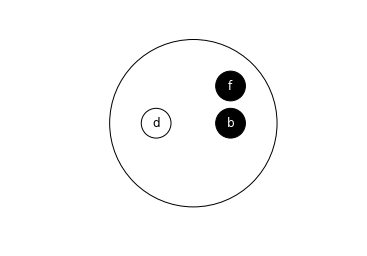
\includegraphics[width=0.6\textwidth]{img/drawing_population.png}
    \end{center}
    \caption{Drawing of population $p(d,fb)$ created by the DN library.}
    \label{fig:drawing_pop}
\end{figure}

The same idea works for a whole DN.
After defining a DarwinianNetwork, the user can call \emph{draw\_dn} passing the DN object.
Figure \ref{fig:drawing_dn} shows one example of the drawing of a DN as generated by the DN library.

\begin{figure}[hbt]
    \begin{center}
        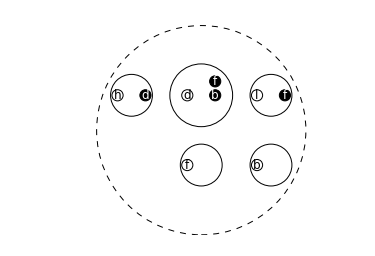
\includegraphics[width=0.6\textwidth]{img/drawing_dn.png}
    \end{center}
    \caption{Drawing of the DN $\{p(h,d), p(l,f), p(f), p(b), p(d,fb)\}$ created by the DN library.}
    \label{fig:drawing_dn}
\end{figure}

\section{Usage}
\label{sec:system:sec3}

The use of the two main classes in DN library is introduced now.
The Population class is defined exactly like a Potential, since it inherits from that class.
But the left and right hand side argument names are replaced by combative and docile, respectively.
Two methods are also exposed for quick references: combative and docile, which returns the respective informations for that Population.
A helper method called \emph{from\_potential} is also available in order to convert a Potential object to a Population one.
Moreover, merge receives another Population as argument, while replicate receives a list of variables which will be marginalized from the Population.

The DarwinianNetwork class has a list member where all the Populations are hold.
The methods \emph{add\_population} and \emph{delete\_population} are used for adding and deleting Population, respectively, from the list of Populations
This class has no constructor and the list of Populations is used to simulate the multi-set definition of DNs.
